\begin{figure}[tbp]
\centering
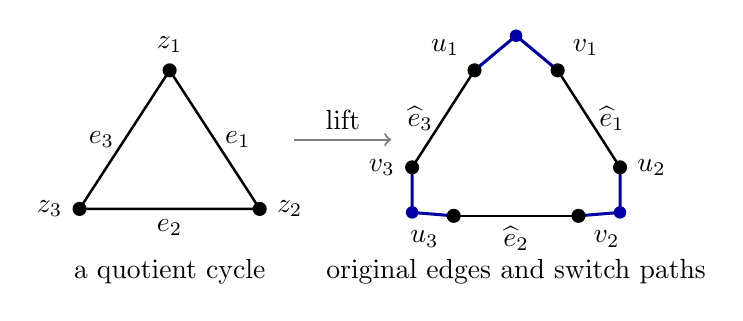
\begin{tikzpicture}[x=0.88cm,y=0.88cm,
  original/.style={line width=0.9pt},
  route/.style={line width=1.1pt,blue!65!black},
  vertex/.style={circle,fill=black,inner sep=1.8pt},
  inside/.style={circle,fill=blue!65!black,inner sep=1.6pt}]
\coordinate (z1) at (0,1.8);
\coordinate (z2) at (1.3,-0.2);
\coordinate (z3) at (-1.3,-0.2);
\draw[original] (z1)--node[right] {$e_1$}(z2)--node[below] {$e_2$}(z3)--node[left] {$e_3$}(z1);
\node[vertex,label=above:$z_1$] at (z1) {};
\node[vertex,label=right:$z_2$] at (z2) {};
\node[vertex,label=left:$z_3$] at (z3) {};
\node at (0,-1.1) {a quotient cycle};
\draw[->,gray,thick] (1.8,0.8)--(3.2,0.8);
\node[above] at (2.5,0.8) {lift};
\coordinate (u1) at (4.4,1.8);
\coordinate (v1) at (5.6,1.8);
\coordinate (u2) at (6.5,0.4);
\coordinate (v2) at (5.9,-0.3);
\coordinate (u3) at (4.1,-0.3);
\coordinate (v3) at (3.5,0.4);
\draw[original] (v1)--node[right] {$\widehat e_1$}(u2);
\draw[original] (v2)--node[below] {$\widehat e_2$}(u3);
\draw[original] (v3)--node[left] {$\widehat e_3$}(u1);
\draw[route] (u1)--(5,2.3)--(v1);
\draw[route] (u2)--(6.5,-0.25)--(v2);
\draw[route] (u3)--(3.5,-0.25)--(v3);
\node[inside] at (5,2.3) {};
\node[inside] at (6.5,-0.25) {};
\node[inside] at (3.5,-0.25) {};
\node[vertex,label=above left:$u_1$] at (u1) {};
\node[vertex,label=above right:$v_1$] at (v1) {};
\node[vertex,label=right:$u_2$] at (u2) {};
\node[vertex,label=below right:$v_2$] at (v2) {};
\node[vertex,label=below left:$u_3$] at (u3) {};
\node[vertex,label=left:$v_3$] at (v3) {};
\node at (5,-1.1) {original edges and switch paths};
\end{tikzpicture}
\caption{Lifting a quotient cycle, schematically. The fiber at \(z_j\)
contains \(u_j,v_j\); when they differ, a reserved path (blue) joins
them. The black edges are the unique original representatives of the
quotient edges. Every path interior avoids all black-edge endpoints,
and the interiors are pairwise disjoint for this cycle. Each blue
path is drawn with one internal vertex only for illustration; its
actual length may differ. A visit with \(u_j=v_j\) requires no path.}
\label{fig:cycle-lifting}
\end{figure}
